\chapter{PCA on spectral data}
\label{ch:spectral-PCA}

\begin{wrapfigure}{o}{0.7\textwidth}
    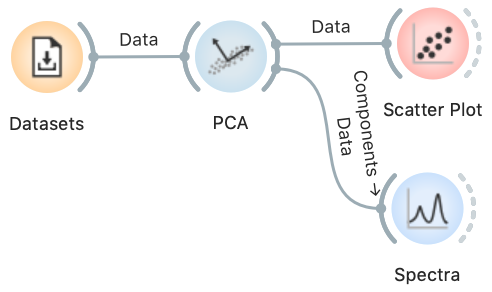
\includegraphics[scale=0.4]{workflow1.png}
\end{wrapfigure}

In this lesson we will explore the capabilities of \mutation\ for principal component analysis (PCA) on spectroscopy data. As usual, we will use the Liver Spectroscopy dataset. Connect \widget{Datasets} to the \widget{PCA} widget, choose the first 5 principal components and then connect \widget{PCA}'s default output, ``Data'', into the \widget{Scatter Plot}.

We see that the first two principal components separate majority compounds in that part of the tissue well.

\begin{figure*}[h]
\centering
\infinitewidthbox{
  \stackinset{r}{-0.35\linewidth}{t}{+0.1\linewidth}
  {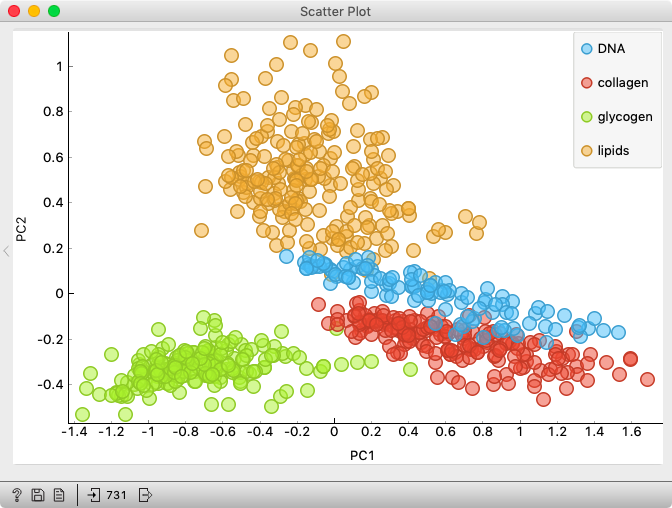
\includegraphics[scale=0.4]{scatterplot.png}}
  {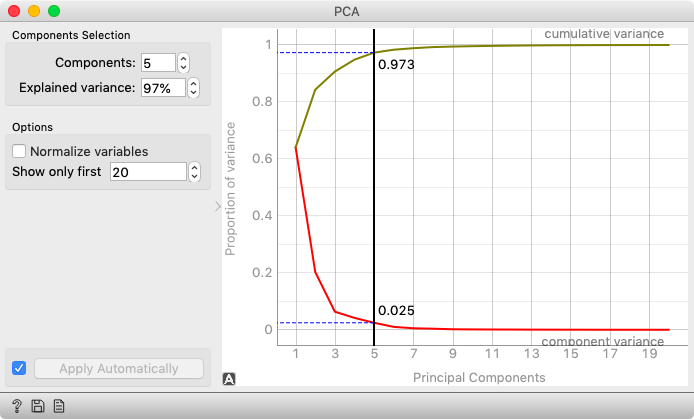
\includegraphics[scale=0.4]{pca.png}}
  \hspace{6cm}
  }
\caption{We chose not to normalize variables in \widget{PCA}. Why?}

\end{figure*}

\begin{wrapfigure}{o}{0.8\textwidth}
  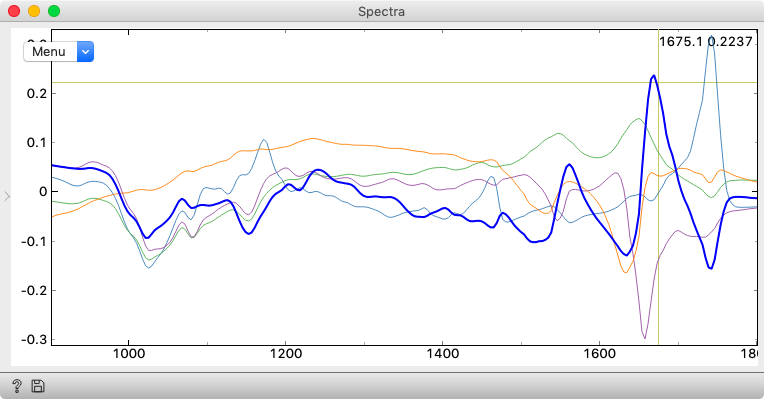
\includegraphics[width=0.8\textwidth]{components.png}%
  \caption{The curve under the cursor is highlighted. A tooltip will appear after some time. If clicked, the curve will be selected.}
\end{wrapfigure}

To see what different principal components represent, connect \widget{PCA’s} ``Components'' output (be careful, \widget{PCA} has 4 outputs) into \widget{Spectra}. Wondering which principal component is highlighted in the following screenshot? Wait for the tooltip...

\clearpage

Let's extend our workflow. If we connect the \widget{PCA} (``Transformed Data'' output) to \widget{Spectra}, we can see each transformed spectrum on a line plot. As we can see, some classes have outliers.

\begin{wrapfigure}{o}{0.9\textwidth}
    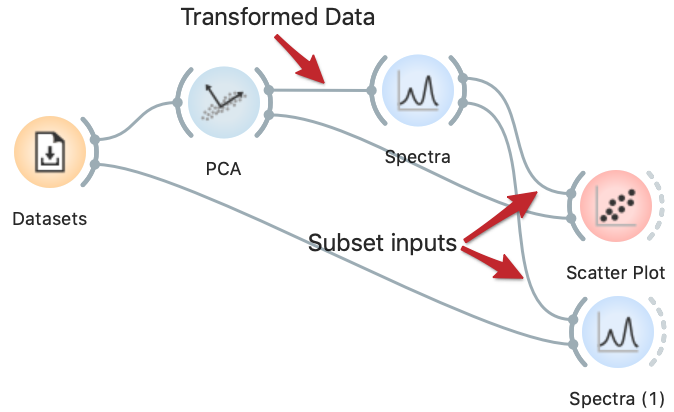
\includegraphics[scale=0.4]{workflow2.png}
\end{wrapfigure}

To find out more about a particular outlier, we can select it in the \widget{Spectra} widget: move your mouse cursor to a curve---it will be highlighted—-and click it. The selected curve changes to a dotted line and is sent to the output.

Then, connect the \widget{Spectra} widget to the \widget{Scatter Plot} and the \widget{Spectra (1)} widgets' ``Data Subset'' inputs; these widgets will need two inputs to function as shown, the subset coming from the selection in \widget{Spectra} and the whole data set. Now we can see the selected outlier in the original space (\widget{Spectra (1)} widget) and in the space of principal components (\widget{Scatter Plot}), both in the context of all spectra from the data set.

\begin{figure*}[h]
  \centering
  \begin{tabular}{ c  c }
      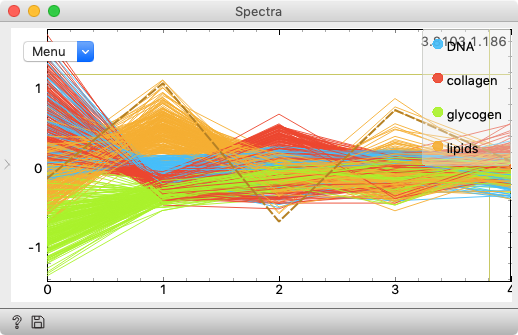
\includegraphics[scale=0.4]{selection-spectra.png}  & 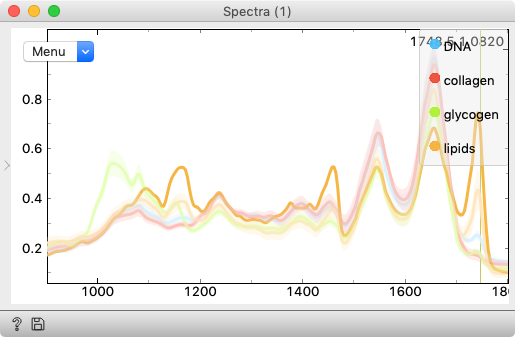
\includegraphics[scale=0.4]{subset-spectra.png} \\
      & 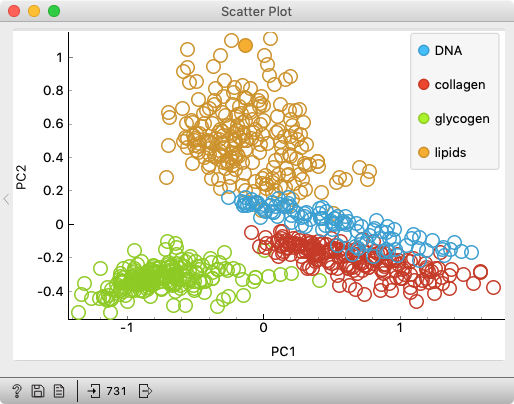
\includegraphics[scale=0.4]{subset-scatterplot.png}
  \end{tabular}
  \vspace{0.3cm}
  \caption{The selected spectrum's curve on the left is drawn with a dashed line and the corresponding original spectrum is highlighted on the right. The \widget{Scatter Plot} shows the position of the selected spectrum in the PCA space.}
\end{figure*}
